\chapter{Vyhodnocení detektorů stop v pevné fázi (praktická část)}
\section{Metodika}\label{sec:praktickaCast_metodika}
NPI používá HARZLAS TD-1 a od roku 2016 i TASTRAK. HARZLAS TD-1 je leptán 18 hodin za teploty 70 $^{\circ}$C v 5 N koncentrovaném roztoku NaOH; odleptaná vrstva je kolem 15,3 $\mu$m. Většinou je analyzována plocha o velikosti 0,09 cm$^2$. Detektor je tlustý 0.9 mm. TASTRAK se leptá dvoufázově: první fáze trvá 6 hodin a jsou při ní zobrazeny stopy vytvořené částicemi s velkým $\mathit{LET}$; při druhé fázi, která trvá dalších 9 hodin, se zobrazí i stopy pocházejících od částic s nižším $\mathit{LET}$. Celkový čas leptání je tedy 15 hodin. Buď se postupuje postupným leptáním (6 hodin leptání, vyhodnocení, 9 hodin leptání, vyhodnocení), nebo se část detektoru leptá 6 hodin a část 15 hodin, tudíž
detektor lze vyhodnotit najednou. Detektor se leptá při 70 $^{\circ}$C v 6,25 N koncentrovaném roztoku NaOH, odleptaná vrstva je tlustá 7,5/20,1 $\mu$m; zpravidla se analyzuje plocha o velikosti 0,5 cm$^2$ (v obou případech) z důvodu zajištění dostatečné statistiky. Po leptání následuje u obou detektorů nasnímání stop lineárním snímacím zařízením s vysokým rozlišením (které je součástí mikroskopu HSP-1000,~\cite{dosis_HSP1000}), poté jsou snímky se stopami analyzovány programem HspFit.

Zatímco HARZLAS TD-1 detekuje částice s $\LET$ vyšším než 7 keV/$\mu$m, TASTRAK má detekční práh 20 keV/$\mu$m. Na druhou stranu TASTRAK má vyšší rozsah měřitelných $\LET$ a díky leptání per partes detekuje s mnohem větší účinností částice s vyšším $\LET$ než HARZLAS TD-1~\cite{cesky}.
\newpage
%V tab. \ref{tab:praktickaCast_rozsahyLET} jsou rozsahy měřitelných $\LET$, tj. částice s $\LET$ v tomto intervalu můžeme zahrnout do výpočtů dávky, $\LET$ spektra atd.
%\begin{table}[H]
  %\centering
  %\caption{Rozsah měřitelných $\LET$ daného detektoru.~\cite{thesisKPBrabcova, cesky}}
  %\label{tab:praktickaCast_rozsahyLET}
  %\begin{tabular}{lll}
	%\toprule
	%Materiál & Rozsah $\LET$ [keV/$\mu$m]\\
	%\midrule
	%HARZLAS TD-1& 7 -- 340\\
	%TASTRAK& 20 -- 450\\
	%\bottomrule
  %\end{tabular}
%\end{table}
\section{Vyhodnocení}
\begin{wrapfigure}{r}{0.42\textwidth}
%\begin{figure}[h]
  \centering
  %\vspace{-20pt}
  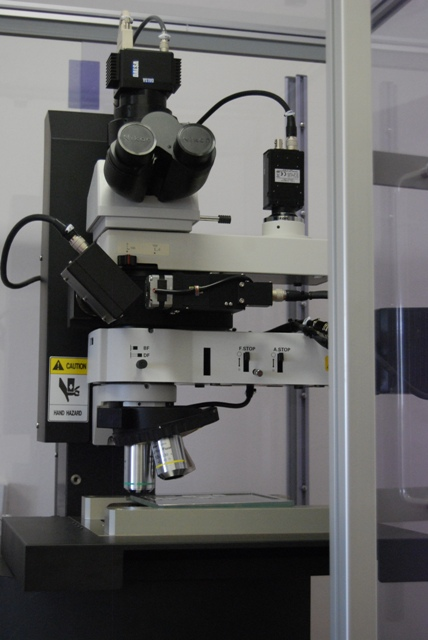
\includegraphics[width=0.4\textwidth]{praktickaCast_mikroskop}
  %\vspace{-20pt}
  \caption{Vysoko rychlostní optický mikroskop HSP-1000.~\cite{dosis_HSP1000}}
  \label{fig:praktickaCast_mikroskop}
  \vspace{-10pt}
%\end{figure}
\end{wrapfigure}
V praktické části bakalářské práce byly vyhodnoceny tři detektory stop osmé sady experimentu DOSIS3D. Detektory byly umístěny v prvním, druhém a třetím PDP. Jedná se o detektory z materiálu Tastrak, které byly leptány 6 hodin, tj. zobrazené stopy jsou původem od částic s krátkým dosahem a vyšším LET.

Na obr.~\ref{fig:praktickaCast_mikroskop} je mikroskopický systém HSP-1000 (neúplný, chybí počítač, který systém řídí) pomocí něhož byl povrch detektorů nasnímán v dostatečném přiblížení.

Vyhodnocovat jsem započal analýzou stop v programu HspFit. Tento program sám vyhodnotí a zaznamená při dobrém nastavení určitých parametrů většinu stop, zbytek se musí označit ručně, což je zdlouhavá práce. Stopy se zaznamenávají tak, že se jejich okraj fituje elipsou, přičemž parametry fitu představují osy elipsy (hlavní $a$ a vedlejší $b$). V případě špatného automatického fitu lze proklad opravit ručně. Na obr.~\ref{fig:praktickaCast_hspfit} vidíme okno programu HspFit, zeleně jsou označeny stopy zaznamenané počítačem, fialově stopy zaznamenané uživatelem. Dále lze pozorovat, že některé stopy ještě zaznamenány nebyly. 
\begin{figure}[ht]
  \centering
  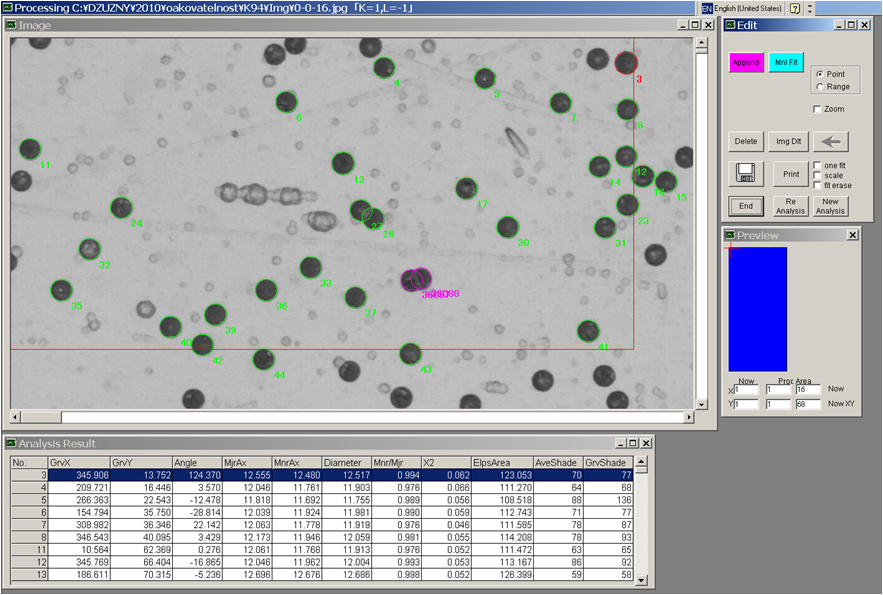
\includegraphics[width=0.85\textwidth]{praktickaCast_hspfit}
  \caption{Okno programu HspFit; zeleně jsou označeny fity vygenerované počítačem a fialově fity vytvořené uživatelem.~\cite{dosis_HSP1000}}
  \label{fig:praktickaCast_hspfit}
\end{figure}

V obr. \ref{fig:praktickaCast_stopy} jsou uvedeny jednotlivé snímky z povrchu náhodně vybraného detektoru. V (a) je snímek, který obsahuje čisté stopy; v (b) ukazuje červená šipka poškození materiálu nepocházející od ozáření ionizujícím zářením, které by mohl neznalý uživatel vyhodnotit jako vícero stop; v (c) taktéž ukazuje červená šipka poškození materiálu jiného charakteru. Obr.~\ref{fig:praktickaCast_stopyPoskozeni} pak ukazuje snímky, na nichž je naskenována plocha, která byla fyzicky znehodnocena člověkem (označení detektoru vyrytím X). 

Osy všech elips byly spolu s dalšími parametry fitů (např. sklon elipsy) uloženy v souboru s příponou .nap. Tato data byla zpracována skriptem napsaném v programovacím jazyce Python, jehož výstupem jsou tři soubory. První soubor obsahuje údaje o poloze stopy, os fitované elipsy, poměru leptacích rychlostí $V$, korekčním součiniteli $k_{\theta}$, lineárním přenosu energie $\LET$, dávce a dávkovém ekvivalentu každé stopy. Druhý soubor obsahuje celkovou dávku a dávkový ekvivalent, které se absorbovaly v detektoru i s jejich příkony. Třetí soubor obsahuje data potřebná k vytvoření diferenciálních $\LET$ spekter; z těchto dat jsem pomocí programu Gnuplot vytvořil grafy \ref{fig:praktickaCast_LETcetnost}, \ref{fig:praktickaCast_LETfluence}, \ref{fig:praktickaCast_LETdavka}
a \ref{fig:praktickaCast_LETdavkEkvivalent}. Skript vypočítává pro každou částici $V$ z hodnot $a,b$ (vztah \eqref{eq:pomerLepRychlosti}, tloušťka odleptané vrstvy je $7,5$
$\mu$m) a následně $\LET$ dané částice z $V$ pomocí kalibrační křivky pro TASTRAK leptaný 6 hodin \eqref{eq:kalibracniKrivkaSestHod}.
\begin{align}
  \LET(V) &= -99,8424+125,00172  V-15,28166  V^2+2,04636  V^3\,,\label{eq:kalibracniKrivkaSestHod}
  %\LET(V) &= -96,35071+114,90343  V-7,77194  V^2+1,27248  V^3\quad\text{(15 hod)},\label{eq:kalibracniKrivkaPatnactHod}
\end{align}
kde $\LET$ vychází v keV/$\mu$m; závislost byla přebrána z \cite{ssntd}. Kalibrační křivka je také k nahlédnutí na obr. \ref{fig:praktickaCast_kalibracniKrivky}.
\begin{figure}[ht]
  \centering
  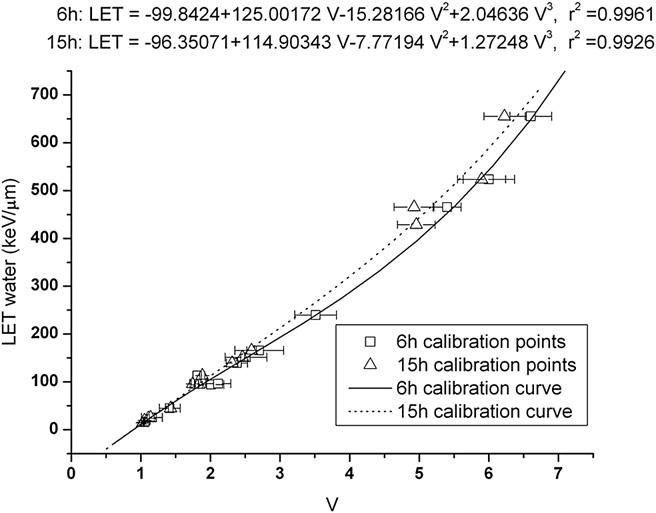
\includegraphics[width=0.7\textwidth]{praktickaCast_kalibracniKrivky.jpg}
  \caption{Kalibrační křivky pro TASTRAK leptaný 6, resp. 15 hodin. Obrázek obsahuje i kalibrační body. Kalibrační křivky pocházejí od MTA EK, \cite{ssntd}.}
  \label{fig:praktickaCast_kalibracniKrivky}
\end{figure}
Z $\LET$ všech částic jsou dále vypočítány dávka a dávkový ekvivalent dle vztahů \eqref{eq:Davka} a \eqref{eq:EkvDavka}. Díky známému času doby měření můžeme určit příkony těchto veličin, tj. $\dot{D}, \dot{H}$.

%Tab. \ref{tab:praktickaCast_davkyVysledky} obsahuje hledané celkové dávky a dávkové ekvivalenty; do vyhodnocení nebyly zahrnuty stopy s $\LET>1000$ (kvůli rozsahu kalibrační křivky). Na obr. \ref{fig:praktickaCast_LETspektra} jsou $\LET$ spektra získaná z vyhodnocených detektorů.

Původní Python skript, který jsem obdržel od vedoucí práce, neposkytoval data pro $\LET$ spektra a nevypočítával $\dot{D},\dot{H}$. Pro tyto účely jsem ho musel dopsat. 
%osmá sada
\begin{table}[h]
  \centering
  \caption{Celkové dávky $D$ a dávkové ekvivalenty $H$ určené vyhodnocovanými detektory.}
  \label{tab:praktickaCast_davkyVysledky}
  \begin{tabular}{lll}
	\toprule
	PDP&$D$ [mGy]&$H$ [mSv]\\
	\midrule
	%1&5,31501450067&88,2754298605\\
	%2&5,068573344&92,5692674847\\
	%3&4,31129592097&75,4191405129\\
	1&$5\pm1$&$90\pm20$\\
	2&$5\pm1$&$90\pm20$\\
	3&$4\pm1$&$90\pm20$\\
	\bottomrule
  \end{tabular}
\end{table}
\begin{figure}[h]
  \centering
  \begin{subfigure}{0.7\textwidth}
	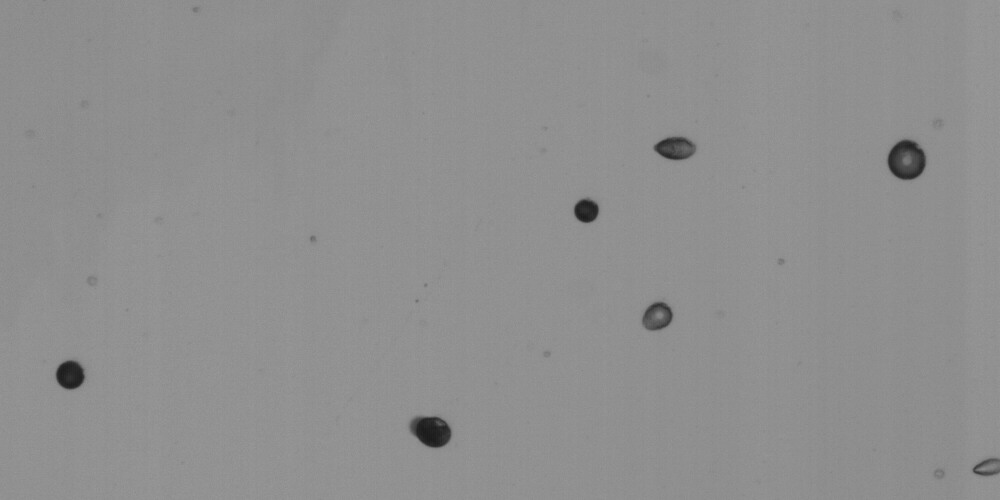
\includegraphics[width=\textwidth]{praktickaCast_stopyOK.jpg}
	\caption{}
  \end{subfigure}
  \begin{subfigure}{0.7\textwidth}
	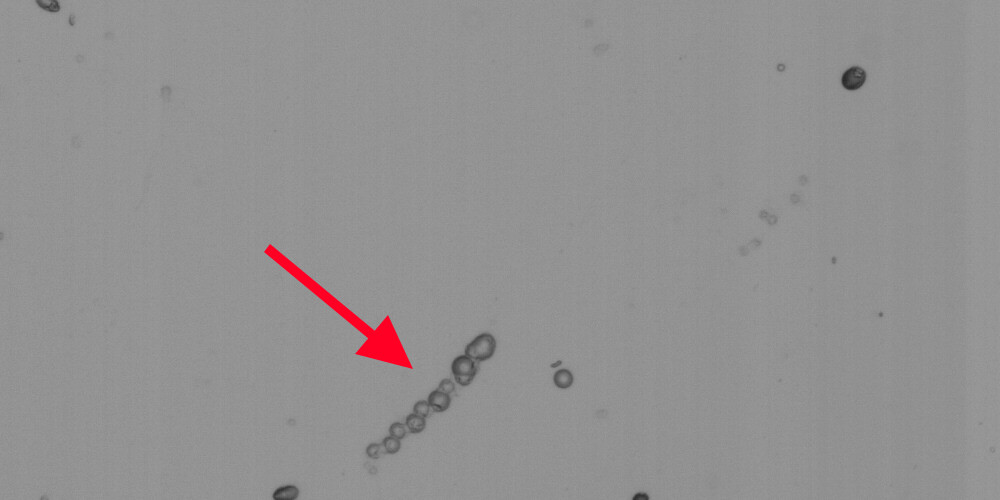
\includegraphics[width=\textwidth]{praktickaCast_stopyNeniStopa1.jpg}
	\caption{}
  \end{subfigure}
  \begin{subfigure}{0.7\textwidth}
	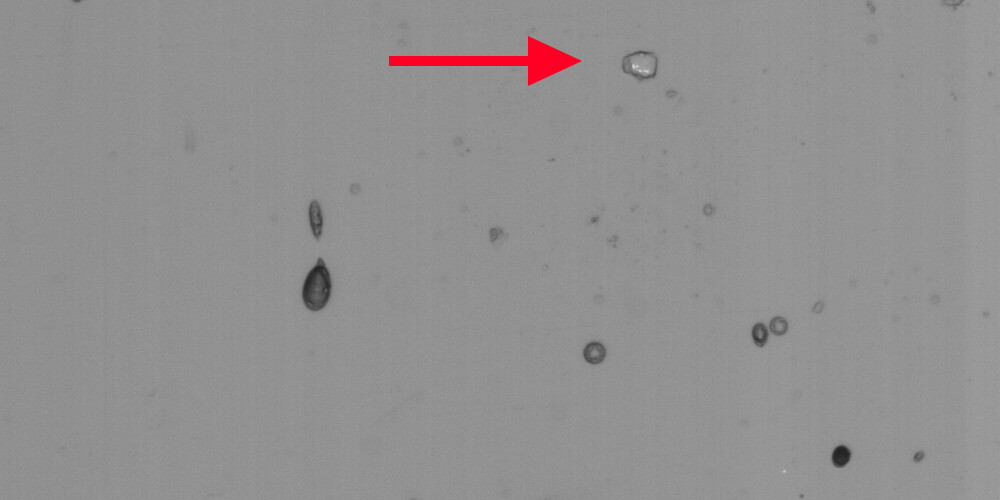
\includegraphics[width=\textwidth]{praktickaCast_stopyNeniStopa2.jpg}
	\caption{}
  \end{subfigure}
  \caption{Příklad naskenovaných snímků jednoho detektoru. V (a) jsou vidět normální stopy, v (b) a (c) naopak červené šipky ukazují na poškození materiálu, která nevznikla působením ionizujícího záření.}
  \label{fig:praktickaCast_stopy}
\end{figure}
\begin{figure}[h]
  \centering
  \begin{subfigure}{0.7\textwidth}
	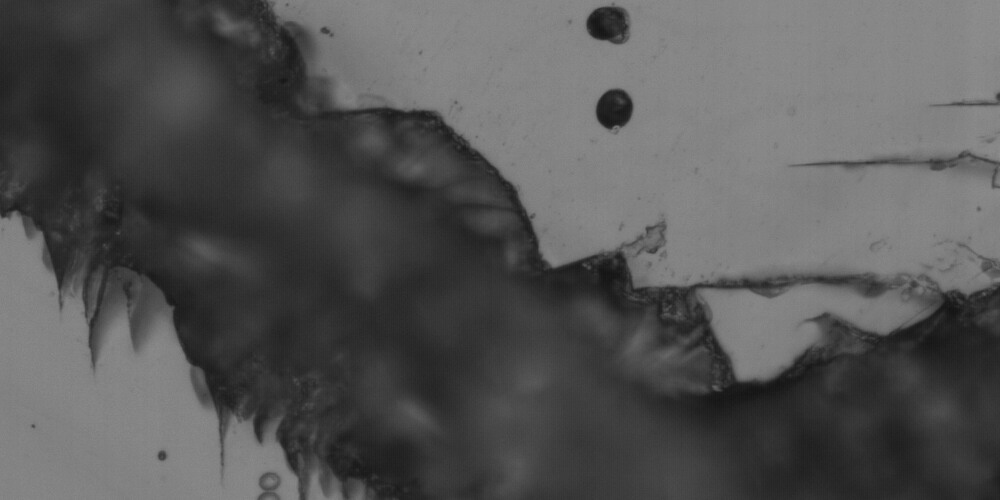
\includegraphics[width=\textwidth]{praktickaCast_stopyPoskozeni1.jpg}
	\caption{}
  \end{subfigure}
  \begin{subfigure}{0.7\textwidth}
	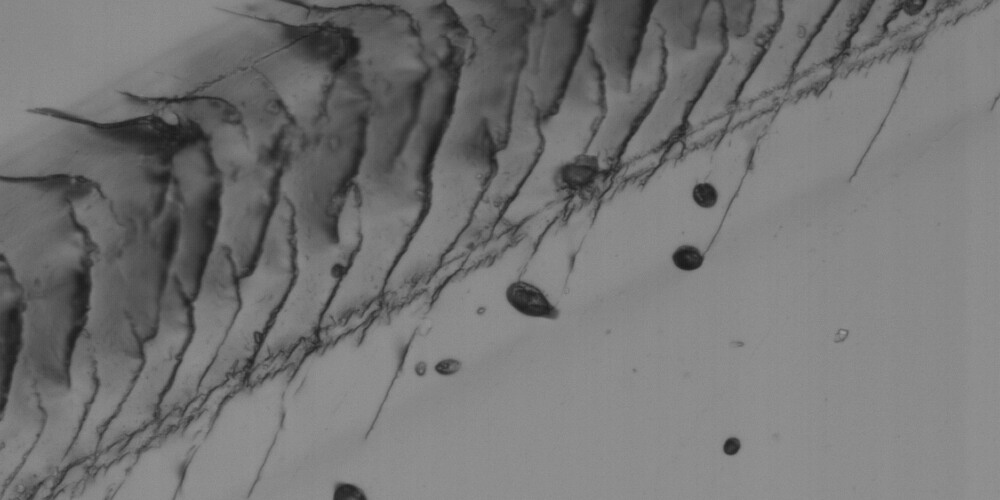
\includegraphics[width=\textwidth]{praktickaCast_stopyPoskozeni2.jpg}
	\caption{}
  \end{subfigure}
  \caption{Naskenované snímky zobrazující poškozené části plochy detektoru vyrytím značky X.}
  \label{fig:praktickaCast_stopyPoskozeni}
\end{figure}
\begin{figure}[h]
  \centering
	\centering
	% GNUPLOT: LaTeX picture with Postscript
\begingroup
  \makeatletter
  \providecommand\color[2][]{%
    \GenericError{(gnuplot) \space\space\space\@spaces}{%
      Package color not loaded in conjunction with
      terminal option `colourtext'%
    }{See the gnuplot documentation for explanation.%
    }{Either use 'blacktext' in gnuplot or load the package
      color.sty in LaTeX.}%
    \renewcommand\color[2][]{}%
  }%
  \providecommand\includegraphics[2][]{%
    \GenericError{(gnuplot) \space\space\space\@spaces}{%
      Package graphicx or graphics not loaded%
    }{See the gnuplot documentation for explanation.%
    }{The gnuplot epslatex terminal needs graphicx.sty or graphics.sty.}%
    \renewcommand\includegraphics[2][]{}%
  }%
  \providecommand\rotatebox[2]{#2}%
  \@ifundefined{ifGPcolor}{%
    \newif\ifGPcolor
    \GPcolortrue
  }{}%
  \@ifundefined{ifGPblacktext}{%
    \newif\ifGPblacktext
    \GPblacktexttrue
  }{}%
  % define a \g@addto@macro without @ in the name:
  \let\gplgaddtomacro\g@addto@macro
  % define empty templates for all commands taking text:
  \gdef\gplbacktext{}%
  \gdef\gplfronttext{}%
  \makeatother
  \ifGPblacktext
    % no textcolor at all
    \def\colorrgb#1{}%
    \def\colorgray#1{}%
  \else
    % gray or color?
    \ifGPcolor
      \def\colorrgb#1{\color[rgb]{#1}}%
      \def\colorgray#1{\color[gray]{#1}}%
      \expandafter\def\csname LTw\endcsname{\color{white}}%
      \expandafter\def\csname LTb\endcsname{\color{black}}%
      \expandafter\def\csname LTa\endcsname{\color{black}}%
      \expandafter\def\csname LT0\endcsname{\color[rgb]{1,0,0}}%
      \expandafter\def\csname LT1\endcsname{\color[rgb]{0,1,0}}%
      \expandafter\def\csname LT2\endcsname{\color[rgb]{0,0,1}}%
      \expandafter\def\csname LT3\endcsname{\color[rgb]{1,0,1}}%
      \expandafter\def\csname LT4\endcsname{\color[rgb]{0,1,1}}%
      \expandafter\def\csname LT5\endcsname{\color[rgb]{1,1,0}}%
      \expandafter\def\csname LT6\endcsname{\color[rgb]{0,0,0}}%
      \expandafter\def\csname LT7\endcsname{\color[rgb]{1,0.3,0}}%
      \expandafter\def\csname LT8\endcsname{\color[rgb]{0.5,0.5,0.5}}%
    \else
      % gray
      \def\colorrgb#1{\color{black}}%
      \def\colorgray#1{\color[gray]{#1}}%
      \expandafter\def\csname LTw\endcsname{\color{white}}%
      \expandafter\def\csname LTb\endcsname{\color{black}}%
      \expandafter\def\csname LTa\endcsname{\color{black}}%
      \expandafter\def\csname LT0\endcsname{\color{black}}%
      \expandafter\def\csname LT1\endcsname{\color{black}}%
      \expandafter\def\csname LT2\endcsname{\color{black}}%
      \expandafter\def\csname LT3\endcsname{\color{black}}%
      \expandafter\def\csname LT4\endcsname{\color{black}}%
      \expandafter\def\csname LT5\endcsname{\color{black}}%
      \expandafter\def\csname LT6\endcsname{\color{black}}%
      \expandafter\def\csname LT7\endcsname{\color{black}}%
      \expandafter\def\csname LT8\endcsname{\color{black}}%
    \fi
  \fi
    \setlength{\unitlength}{0.0500bp}%
    \ifx\gptboxheight\undefined%
      \newlength{\gptboxheight}%
      \newlength{\gptboxwidth}%
      \newsavebox{\gptboxtext}%
    \fi%
    \setlength{\fboxrule}{0.5pt}%
    \setlength{\fboxsep}{1pt}%
\begin{picture}(7936.00,5102.00)%
    \gplgaddtomacro\gplbacktext{%
      \csname LTb\endcsname%
      \put(946,704){\makebox(0,0)[r]{\strut{}$1$}}%
      \csname LTb\endcsname%
      \put(946,2082){\makebox(0,0)[r]{\strut{}$10$}}%
      \csname LTb\endcsname%
      \put(946,3459){\makebox(0,0)[r]{\strut{}$100$}}%
      \csname LTb\endcsname%
      \put(946,4837){\makebox(0,0)[r]{\strut{}$1000$}}%
      \csname LTb\endcsname%
      \put(1078,484){\makebox(0,0){\strut{}$10$}}%
      \csname LTb\endcsname%
      \put(4309,484){\makebox(0,0){\strut{}$100$}}%
      \csname LTb\endcsname%
      \put(7539,484){\makebox(0,0){\strut{}$1000$}}%
    }%
    \gplgaddtomacro\gplfronttext{%
      \csname LTb\endcsname%
      \put(176,2770){\rotatebox{-270}{\makebox(0,0){\strut{}$N$ [-]}}}%
      \put(4308,154){\makebox(0,0){\strut{}$\mathit{LET}$ [keV/$\mu$m]}}%
      \csname LTb\endcsname%
      \put(6624,4616){\makebox(0,0)[r]{\strut{}PDP1}}%
      \csname LTb\endcsname%
      \put(6624,4301){\makebox(0,0)[r]{\strut{}PDP2}}%
      \csname LTb\endcsname%
      \put(6624,3986){\makebox(0,0)[r]{\strut{}PDP3}}%
    }%
    \gplbacktext
    \put(0,0){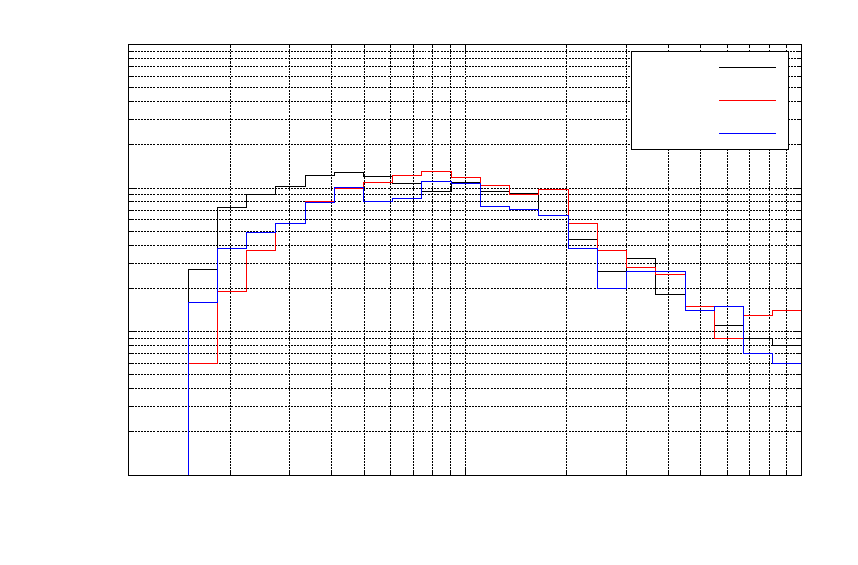
\includegraphics{LETspektrumCetnost}}%
    \gplfronttext
  \end{picture}%
\endgroup

	\caption{}
	\label{fig:praktickaCast_LETcetnost}
\end{figure}
\begin{figure}[h]
  \centering
	\centering
	% GNUPLOT: LaTeX picture with Postscript
\begingroup
  \makeatletter
  \providecommand\color[2][]{%
    \GenericError{(gnuplot) \space\space\space\@spaces}{%
      Package color not loaded in conjunction with
      terminal option `colourtext'%
    }{See the gnuplot documentation for explanation.%
    }{Either use 'blacktext' in gnuplot or load the package
      color.sty in LaTeX.}%
    \renewcommand\color[2][]{}%
  }%
  \providecommand\includegraphics[2][]{%
    \GenericError{(gnuplot) \space\space\space\@spaces}{%
      Package graphicx or graphics not loaded%
    }{See the gnuplot documentation for explanation.%
    }{The gnuplot epslatex terminal needs graphicx.sty or graphics.sty.}%
    \renewcommand\includegraphics[2][]{}%
  }%
  \providecommand\rotatebox[2]{#2}%
  \@ifundefined{ifGPcolor}{%
    \newif\ifGPcolor
    \GPcolortrue
  }{}%
  \@ifundefined{ifGPblacktext}{%
    \newif\ifGPblacktext
    \GPblacktexttrue
  }{}%
  % define a \g@addto@macro without @ in the name:
  \let\gplgaddtomacro\g@addto@macro
  % define empty templates for all commands taking text:
  \gdef\gplbacktext{}%
  \gdef\gplfronttext{}%
  \makeatother
  \ifGPblacktext
    % no textcolor at all
    \def\colorrgb#1{}%
    \def\colorgray#1{}%
  \else
    % gray or color?
    \ifGPcolor
      \def\colorrgb#1{\color[rgb]{#1}}%
      \def\colorgray#1{\color[gray]{#1}}%
      \expandafter\def\csname LTw\endcsname{\color{white}}%
      \expandafter\def\csname LTb\endcsname{\color{black}}%
      \expandafter\def\csname LTa\endcsname{\color{black}}%
      \expandafter\def\csname LT0\endcsname{\color[rgb]{1,0,0}}%
      \expandafter\def\csname LT1\endcsname{\color[rgb]{0,1,0}}%
      \expandafter\def\csname LT2\endcsname{\color[rgb]{0,0,1}}%
      \expandafter\def\csname LT3\endcsname{\color[rgb]{1,0,1}}%
      \expandafter\def\csname LT4\endcsname{\color[rgb]{0,1,1}}%
      \expandafter\def\csname LT5\endcsname{\color[rgb]{1,1,0}}%
      \expandafter\def\csname LT6\endcsname{\color[rgb]{0,0,0}}%
      \expandafter\def\csname LT7\endcsname{\color[rgb]{1,0.3,0}}%
      \expandafter\def\csname LT8\endcsname{\color[rgb]{0.5,0.5,0.5}}%
    \else
      % gray
      \def\colorrgb#1{\color{black}}%
      \def\colorgray#1{\color[gray]{#1}}%
      \expandafter\def\csname LTw\endcsname{\color{white}}%
      \expandafter\def\csname LTb\endcsname{\color{black}}%
      \expandafter\def\csname LTa\endcsname{\color{black}}%
      \expandafter\def\csname LT0\endcsname{\color{black}}%
      \expandafter\def\csname LT1\endcsname{\color{black}}%
      \expandafter\def\csname LT2\endcsname{\color{black}}%
      \expandafter\def\csname LT3\endcsname{\color{black}}%
      \expandafter\def\csname LT4\endcsname{\color{black}}%
      \expandafter\def\csname LT5\endcsname{\color{black}}%
      \expandafter\def\csname LT6\endcsname{\color{black}}%
      \expandafter\def\csname LT7\endcsname{\color{black}}%
      \expandafter\def\csname LT8\endcsname{\color{black}}%
    \fi
  \fi
    \setlength{\unitlength}{0.0500bp}%
    \ifx\gptboxheight\undefined%
      \newlength{\gptboxheight}%
      \newlength{\gptboxwidth}%
      \newsavebox{\gptboxtext}%
    \fi%
    \setlength{\fboxrule}{0.5pt}%
    \setlength{\fboxsep}{1pt}%
\begin{picture}(7936.00,5102.00)%
    \gplgaddtomacro\gplbacktext{%
      \csname LTb\endcsname%
      \put(946,704){\makebox(0,0)[r]{\strut{}$1$}}%
      \csname LTb\endcsname%
      \put(946,2082){\makebox(0,0)[r]{\strut{}$10$}}%
      \csname LTb\endcsname%
      \put(946,3459){\makebox(0,0)[r]{\strut{}$100$}}%
      \csname LTb\endcsname%
      \put(946,4837){\makebox(0,0)[r]{\strut{}$1000$}}%
      \csname LTb\endcsname%
      \put(1078,484){\makebox(0,0){\strut{}$10$}}%
      \csname LTb\endcsname%
      \put(4309,484){\makebox(0,0){\strut{}$100$}}%
      \csname LTb\endcsname%
      \put(7539,484){\makebox(0,0){\strut{}$1000$}}%
    }%
    \gplgaddtomacro\gplfronttext{%
      \csname LTb\endcsname%
      \put(176,2770){\rotatebox{-270}{\makebox(0,0){\strut{}$\Phi$ [cm$^{-2}$sr$^{-1}$]}}}%
      \put(4308,154){\makebox(0,0){\strut{}$\mathit{LET}$ [keV/$\mu$m]}}%
      \csname LTb\endcsname%
      \put(6624,4616){\makebox(0,0)[r]{\strut{}PDP1}}%
      \csname LTb\endcsname%
      \put(6624,4301){\makebox(0,0)[r]{\strut{}PDP2}}%
      \csname LTb\endcsname%
      \put(6624,3986){\makebox(0,0)[r]{\strut{}PDP3}}%
    }%
    \gplbacktext
    \put(0,0){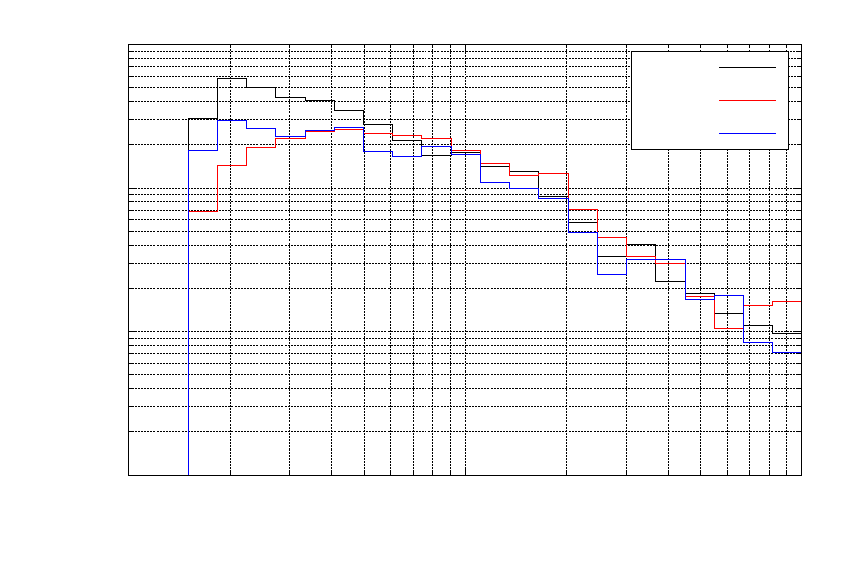
\includegraphics{LETspektrumFluence}}%
    \gplfronttext
  \end{picture}%
\endgroup

	\caption{}
	\label{fig:praktickaCast_LETfluence}
\end{figure}
\begin{figure}[h]
  \centering
	\centering
	% GNUPLOT: LaTeX picture with Postscript
\begingroup
  \makeatletter
  \providecommand\color[2][]{%
    \GenericError{(gnuplot) \space\space\space\@spaces}{%
      Package color not loaded in conjunction with
      terminal option `colourtext'%
    }{See the gnuplot documentation for explanation.%
    }{Either use 'blacktext' in gnuplot or load the package
      color.sty in LaTeX.}%
    \renewcommand\color[2][]{}%
  }%
  \providecommand\includegraphics[2][]{%
    \GenericError{(gnuplot) \space\space\space\@spaces}{%
      Package graphicx or graphics not loaded%
    }{See the gnuplot documentation for explanation.%
    }{The gnuplot epslatex terminal needs graphicx.sty or graphics.sty.}%
    \renewcommand\includegraphics[2][]{}%
  }%
  \providecommand\rotatebox[2]{#2}%
  \@ifundefined{ifGPcolor}{%
    \newif\ifGPcolor
    \GPcolortrue
  }{}%
  \@ifundefined{ifGPblacktext}{%
    \newif\ifGPblacktext
    \GPblacktexttrue
  }{}%
  % define a \g@addto@macro without @ in the name:
  \let\gplgaddtomacro\g@addto@macro
  % define empty templates for all commands taking text:
  \gdef\gplbacktext{}%
  \gdef\gplfronttext{}%
  \makeatother
  \ifGPblacktext
    % no textcolor at all
    \def\colorrgb#1{}%
    \def\colorgray#1{}%
  \else
    % gray or color?
    \ifGPcolor
      \def\colorrgb#1{\color[rgb]{#1}}%
      \def\colorgray#1{\color[gray]{#1}}%
      \expandafter\def\csname LTw\endcsname{\color{white}}%
      \expandafter\def\csname LTb\endcsname{\color{black}}%
      \expandafter\def\csname LTa\endcsname{\color{black}}%
      \expandafter\def\csname LT0\endcsname{\color[rgb]{1,0,0}}%
      \expandafter\def\csname LT1\endcsname{\color[rgb]{0,1,0}}%
      \expandafter\def\csname LT2\endcsname{\color[rgb]{0,0,1}}%
      \expandafter\def\csname LT3\endcsname{\color[rgb]{1,0,1}}%
      \expandafter\def\csname LT4\endcsname{\color[rgb]{0,1,1}}%
      \expandafter\def\csname LT5\endcsname{\color[rgb]{1,1,0}}%
      \expandafter\def\csname LT6\endcsname{\color[rgb]{0,0,0}}%
      \expandafter\def\csname LT7\endcsname{\color[rgb]{1,0.3,0}}%
      \expandafter\def\csname LT8\endcsname{\color[rgb]{0.5,0.5,0.5}}%
    \else
      % gray
      \def\colorrgb#1{\color{black}}%
      \def\colorgray#1{\color[gray]{#1}}%
      \expandafter\def\csname LTw\endcsname{\color{white}}%
      \expandafter\def\csname LTb\endcsname{\color{black}}%
      \expandafter\def\csname LTa\endcsname{\color{black}}%
      \expandafter\def\csname LT0\endcsname{\color{black}}%
      \expandafter\def\csname LT1\endcsname{\color{black}}%
      \expandafter\def\csname LT2\endcsname{\color{black}}%
      \expandafter\def\csname LT3\endcsname{\color{black}}%
      \expandafter\def\csname LT4\endcsname{\color{black}}%
      \expandafter\def\csname LT5\endcsname{\color{black}}%
      \expandafter\def\csname LT6\endcsname{\color{black}}%
      \expandafter\def\csname LT7\endcsname{\color{black}}%
      \expandafter\def\csname LT8\endcsname{\color{black}}%
    \fi
  \fi
    \setlength{\unitlength}{0.0500bp}%
    \ifx\gptboxheight\undefined%
      \newlength{\gptboxheight}%
      \newlength{\gptboxwidth}%
      \newsavebox{\gptboxtext}%
    \fi%
    \setlength{\fboxrule}{0.5pt}%
    \setlength{\fboxsep}{1pt}%
\begin{picture}(7936.00,5102.00)%
    \gplgaddtomacro\gplbacktext{%
      \csname LTb\endcsname%
      \put(946,704){\makebox(0,0)[r]{\strut{}$10$}}%
      \csname LTb\endcsname%
      \put(946,2771){\makebox(0,0)[r]{\strut{}$100$}}%
      \csname LTb\endcsname%
      \put(946,4837){\makebox(0,0)[r]{\strut{}$1000$}}%
      \csname LTb\endcsname%
      \put(1078,484){\makebox(0,0){\strut{}$10$}}%
      \csname LTb\endcsname%
      \put(4309,484){\makebox(0,0){\strut{}$100$}}%
      \csname LTb\endcsname%
      \put(7539,484){\makebox(0,0){\strut{}$1000$}}%
    }%
    \gplgaddtomacro\gplfronttext{%
      \csname LTb\endcsname%
      \put(176,2770){\rotatebox{-270}{\makebox(0,0){\strut{}$D$ [$\mu$Gy]}}}%
      \put(4308,154){\makebox(0,0){\strut{}$\mathit{LET}$ [keV/$\mu$m]}}%
      \csname LTb\endcsname%
      \put(6624,4616){\makebox(0,0)[r]{\strut{}PDP1}}%
      \csname LTb\endcsname%
      \put(6624,4301){\makebox(0,0)[r]{\strut{}PDP2}}%
      \csname LTb\endcsname%
      \put(6624,3986){\makebox(0,0)[r]{\strut{}PDP3}}%
    }%
    \gplbacktext
    \put(0,0){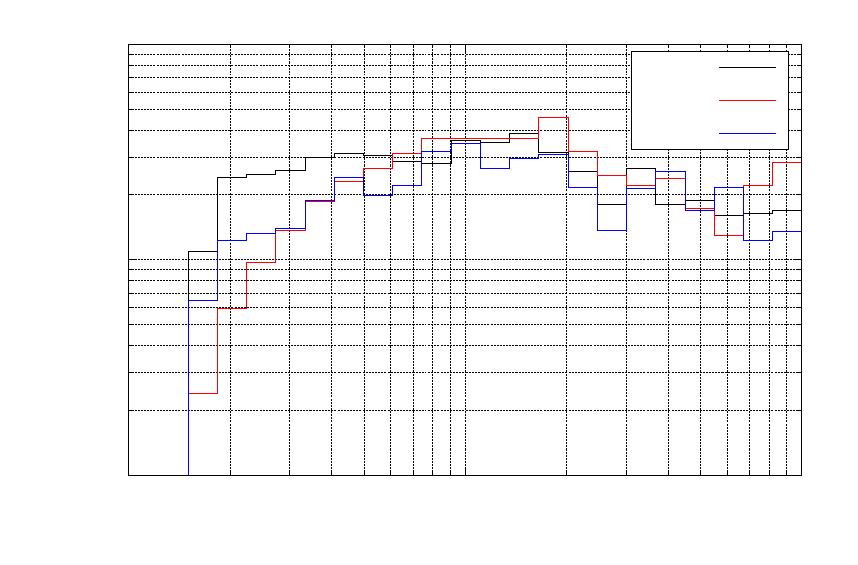
\includegraphics{LETspektrumDavka}}%
    \gplfronttext
  \end{picture}%
\endgroup

	\caption{}
	\label{fig:praktickaCast_LETdavka}
\end{figure}
\begin{figure}[h]
  \centering
	\centering
	% GNUPLOT: LaTeX picture with Postscript
\begingroup
  \makeatletter
  \providecommand\color[2][]{%
    \GenericError{(gnuplot) \space\space\space\@spaces}{%
      Package color not loaded in conjunction with
      terminal option `colourtext'%
    }{See the gnuplot documentation for explanation.%
    }{Either use 'blacktext' in gnuplot or load the package
      color.sty in LaTeX.}%
    \renewcommand\color[2][]{}%
  }%
  \providecommand\includegraphics[2][]{%
    \GenericError{(gnuplot) \space\space\space\@spaces}{%
      Package graphicx or graphics not loaded%
    }{See the gnuplot documentation for explanation.%
    }{The gnuplot epslatex terminal needs graphicx.sty or graphics.sty.}%
    \renewcommand\includegraphics[2][]{}%
  }%
  \providecommand\rotatebox[2]{#2}%
  \@ifundefined{ifGPcolor}{%
    \newif\ifGPcolor
    \GPcolortrue
  }{}%
  \@ifundefined{ifGPblacktext}{%
    \newif\ifGPblacktext
    \GPblacktexttrue
  }{}%
  % define a \g@addto@macro without @ in the name:
  \let\gplgaddtomacro\g@addto@macro
  % define empty templates for all commands taking text:
  \gdef\gplbacktext{}%
  \gdef\gplfronttext{}%
  \makeatother
  \ifGPblacktext
    % no textcolor at all
    \def\colorrgb#1{}%
    \def\colorgray#1{}%
  \else
    % gray or color?
    \ifGPcolor
      \def\colorrgb#1{\color[rgb]{#1}}%
      \def\colorgray#1{\color[gray]{#1}}%
      \expandafter\def\csname LTw\endcsname{\color{white}}%
      \expandafter\def\csname LTb\endcsname{\color{black}}%
      \expandafter\def\csname LTa\endcsname{\color{black}}%
      \expandafter\def\csname LT0\endcsname{\color[rgb]{1,0,0}}%
      \expandafter\def\csname LT1\endcsname{\color[rgb]{0,1,0}}%
      \expandafter\def\csname LT2\endcsname{\color[rgb]{0,0,1}}%
      \expandafter\def\csname LT3\endcsname{\color[rgb]{1,0,1}}%
      \expandafter\def\csname LT4\endcsname{\color[rgb]{0,1,1}}%
      \expandafter\def\csname LT5\endcsname{\color[rgb]{1,1,0}}%
      \expandafter\def\csname LT6\endcsname{\color[rgb]{0,0,0}}%
      \expandafter\def\csname LT7\endcsname{\color[rgb]{1,0.3,0}}%
      \expandafter\def\csname LT8\endcsname{\color[rgb]{0.5,0.5,0.5}}%
    \else
      % gray
      \def\colorrgb#1{\color{black}}%
      \def\colorgray#1{\color[gray]{#1}}%
      \expandafter\def\csname LTw\endcsname{\color{white}}%
      \expandafter\def\csname LTb\endcsname{\color{black}}%
      \expandafter\def\csname LTa\endcsname{\color{black}}%
      \expandafter\def\csname LT0\endcsname{\color{black}}%
      \expandafter\def\csname LT1\endcsname{\color{black}}%
      \expandafter\def\csname LT2\endcsname{\color{black}}%
      \expandafter\def\csname LT3\endcsname{\color{black}}%
      \expandafter\def\csname LT4\endcsname{\color{black}}%
      \expandafter\def\csname LT5\endcsname{\color{black}}%
      \expandafter\def\csname LT6\endcsname{\color{black}}%
      \expandafter\def\csname LT7\endcsname{\color{black}}%
      \expandafter\def\csname LT8\endcsname{\color{black}}%
    \fi
  \fi
    \setlength{\unitlength}{0.0500bp}%
    \ifx\gptboxheight\undefined%
      \newlength{\gptboxheight}%
      \newlength{\gptboxwidth}%
      \newsavebox{\gptboxtext}%
    \fi%
    \setlength{\fboxrule}{0.5pt}%
    \setlength{\fboxsep}{1pt}%
\begin{picture}(7936.00,5102.00)%
    \gplgaddtomacro\gplbacktext{%
      \csname LTb\endcsname%
      \put(1210,704){\makebox(0,0)[r]{\strut{}$10$}}%
      \csname LTb\endcsname%
      \put(1210,1737){\makebox(0,0)[r]{\strut{}$100$}}%
      \csname LTb\endcsname%
      \put(1210,2771){\makebox(0,0)[r]{\strut{}$1000$}}%
      \csname LTb\endcsname%
      \put(1210,3804){\makebox(0,0)[r]{\strut{}$10000$}}%
      \csname LTb\endcsname%
      \put(1210,4837){\makebox(0,0)[r]{\strut{}$100000$}}%
      \csname LTb\endcsname%
      \put(1342,484){\makebox(0,0){\strut{}$10$}}%
      \csname LTb\endcsname%
      \put(4441,484){\makebox(0,0){\strut{}$100$}}%
      \csname LTb\endcsname%
      \put(7539,484){\makebox(0,0){\strut{}$1000$}}%
    }%
    \gplgaddtomacro\gplfronttext{%
      \csname LTb\endcsname%
      \put(176,2770){\rotatebox{-270}{\makebox(0,0){\strut{}$H$ [$\mu$Sv]}}}%
      \put(4440,154){\makebox(0,0){\strut{}$\mathit{LET}$ [keV/$\mu$m]}}%
      \csname LTb\endcsname%
      \put(6624,4616){\makebox(0,0)[r]{\strut{}PDP1}}%
      \csname LTb\endcsname%
      \put(6624,4301){\makebox(0,0)[r]{\strut{}PDP2}}%
      \csname LTb\endcsname%
      \put(6624,3986){\makebox(0,0)[r]{\strut{}PDP3}}%
    }%
    \gplbacktext
    \put(0,0){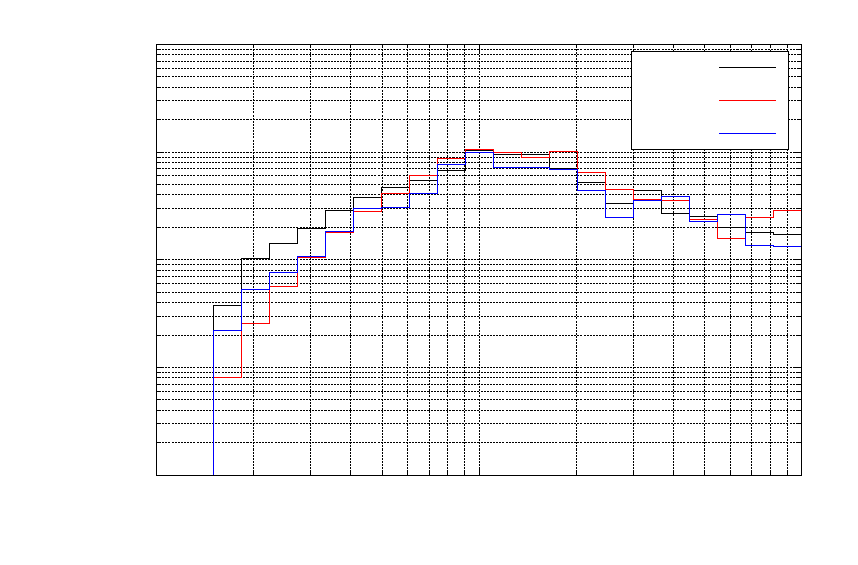
\includegraphics{LETspektrumDavkEkvivalent}}%
    \gplfronttext
  \end{picture}%
\endgroup

	\caption{}
	\label{fig:praktickaCast_LETdavkEkvivalent}
\end{figure}

